\chapter{Das Chlorophyll und sein Abbauprozess}

\section{Der Abbauprozess und seine Bedeutung}

Jedes Jahr werden weltweit schätzungsweise $10^{9}$ Tonnen an Chlorophyll abgebaut. Der Abbauprozess des Chlorophylls ist damit aufgrund der markanten Farbveränderungen einer der visuell am meisten wahrgenommenen biochemischen Vorgänge und kann sogar aus dem All beobachtet werden. \cite{ChlorophyllBreakdown} Die schönen, bunten Farben des Herbstlaubes werden dabei jedoch nicht primär durch die Abbauprodukte des Chlorophylls (im Folgenden Chlorophyll-Kataboliten) hervorgerufen  \cite{DegradationChlorophyll}, da die Endprodukte des Chlorophyllabbaus zumeist farbblos sind. \cite{ChlorophyllBreakdown} Im Folgenden ist immer die Rede vom Abbauprozess in höheren Pflanzen, da gezeigt wurde, dass z. B. marine Lebensformen das Chlorophyll auf einem anderen Wege abbauen und dementsprechend andere Endprodukte vorzufinden sind. \cite{ChlorophyllBreakdown}, \cite{ErsterKatabolit}, \cite{ChlorophyllCataboliteDifferent} Die Abbauprodukte fallen in die Klasse der Phyllobiline (heterocyclische Tetrapyrrole) und sind Anzeichen für Reifung, Seneszenz und Zelltod. Der Abbauprozess wird unter anderem im Rahmen eines Entgiftungsprozesses begangen. \cite{ChlorophyllKatabolitenalsZeichenReifung}

\begin{figure}[!hbtp]
  \centering
  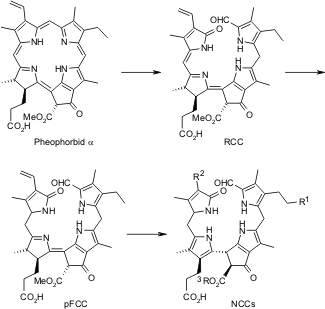
\includegraphics[scale=0.5]{figures/Kapitel2/VWA_Schema_Chlorophyllabbau.png}
  \caption[Abbauprozess des Chlorophylls, Quelle: http://www.organische-chemie.ch/chemie/2007nov/antioxidantien.shtm (Zugegriffen am: 05.11.2017)]{Abbauprozess des Chlorophylls in seneszenten Blättern}
  \label{fig:Chlorophyllabbau}
\end{figure}

Die Struktur eines \gls{Chl-K}en konnte erstmalig im Jahre 1991 aufgeklärt werden. Es handelte sich hierbei um einen \textit{Hv}-\gls{NCC} der Gerste (\textit{Hordeum vulgare}) \cite{ErsterKatabolit}, das Endprodukt eines mehrstufigen Abbauprozesses. 

In den darauffolgenden Jahren fand man heraus, dass das Chlorophyll zuerst in das Pheophorbid a umgewandelt wird. Im nächsten Schritt wird der Makrozyklus oxygenolytisch (an der Reaktion beteiligtes Enzym: Pheo \textit{a} Mono-oxygenase \cite{ChlorophyllCatabolitesEnzyme}) in der nördlichen \textit{meso} Position geöffnet, woraufhin ein \textit{Red Chlorophyll Catabolite} (RCC) entsteht. 
Über einen \textit{primary flourescent Chlorophyll Catabolite} (pFCC) entsteht durch eine nichtenzymatische Isomerisierung ein \gls{NCC}. Thermodynamische Triebkraft dieser Reaktion ist die Rearomatisierung von Ring D. \cite{FCCKatabolit}, \cite{ChlorophyllCatabolites} Die unterschiedlichen Arten von \gls{NCC}s ergeben sich durch Anlagerung der entsprechenden funktionellen Gruppen (z. B. Zuckerring, Hydroxygruppe) an den pFCC. \cite{ChlorophyllCatabolites} 

\section{Nummerierung von Phyllobilinen}

\begin{figure}[!hbtp]
  \centering
  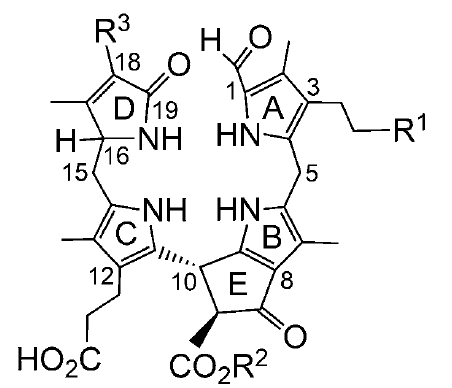
\includegraphics[scale=0.61]{figures/Kapitel2/VWA_Chl-Nummerierung.png}
  \caption[Nummerierung von Phyllobilinen, Quelle: Mathias Scherl]{Positionsangaben und Bezeichnungen der Ringe, die in der restlichen Arbeit für Ausführungen verwendet werden.}
  \label{fig:NummerierungPhyllobiline}
\end{figure}



